Hash tables generalise the simple notion of direct addressing making effective uise of the ability to examine an arbtrary element of an array in $O(1)$ which we know is not affordable when the key universe is big, because it requires space which is proportional to the size of the universe. 
\subsection{Direct Addressing Table}
Suppose for instance that an application needs a synamic set in which each elemtn has a keu drqwn from the universe $U 0 \{0,1,\ldots m-1\} $ where $m$ is not too large and no towo element share the same key (indiex of the direct addressing table).
A direct addressing table is a indexable structure of size $m$ where each key of the universe has a one to one correspondence to one slot of the table. 
Dictionary operations can be performed as follows:

\begin{algorithm}
\Fn{SEARCH (T,k)}{
	$return T[k]$
 }
 \Fn{INSERT (T,x)}{
	$T[tokey(x)] = x$
 }
 \Fn{DELETE (T,x)}{
	$T[tokey(x)] = NIL$
 }
\caption{DIRECT ADDRESSING OPERATIONS}
\end{algorithm}

	\begin{figure}
	\label{fig:directaddressing}
	\centering
		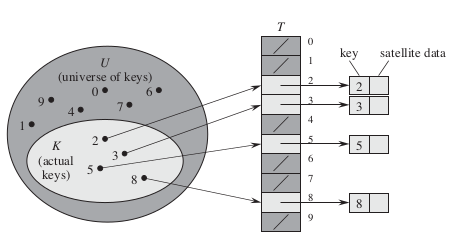
\includegraphics{direct_addressing}
	\end{figure}

where $tokey$ is a function which takes an object $x$ and maps it to an integer in the interval $0\ldots m-1$. Such function is called $hashing function$. 
%---Problem------------
\begin{problem}
\textit{Suppose that a dynamic set S is represented by a direct-address table $T$ of length $m$. Describe a procedure that finds the maximum element of $S$. What is the worst-case performance of your procedure?}.

\begin{solution}
The direct addressing table is not sorted so binary search cannot be used. Only option is a linear scan.
\end{solution}
\end{problem}

Hash tables use addressing with indices as basic idea, but overcome the problem of using large space by using space which is proportional to the number of keys actually stored. The main idea is that we can compute an index from each key to be inserted, in $O(1)$ and use that index as the index of the array location where to store the object. Obviously a because the number of slots is less than the number of possible keys it is possible for two key to be stored at the same location hyelding to a \textit{collision}. There are various effective approach to handle collision which will be describer in the following sections.
In a hash table an element with is stored at slot $h(x)$ where $h$ is an hash function which maps the universe of keys $U$ into slots of the hash table.
\[
h(x): U \mapsto \{0,1,\ldots,m-1\}
\]
with $m$ typically much smaller than $|U|$. The hitch is that (pigeone priciple) two object may be assigned the same slot (they hash to the same slot). This situation is called a \textbf{collision}. There are several tecnquiques to deal with collisions such as 
\begin{enumerate}
\item chaining
\item open addressing
\item linear probing
\item quadratic probing
\item random probing
\end{enumerate}
Of course the best scenario is to avoid collision altogether but since the size of the universe if bigger than the size of the hash table there always exists at least a couple of object which will hash to the same slot. The hash function should, in order to minimize collision as much random as possible (remaining deterministic obviously). The word hash means to mix and it somehow evoke what this function does. It mixes data taken from the object in order to provide a random looking index to be used as an index of the hash table.

\subsection{Collision resolution by chaining}
In chaining, all the elements that hash to the same slot are placed into the same linked-list. The hash table can be viewed, infact, as an array of linked list where each node of the list contains apointer to the object stored.
Dictionary operation can so be performed in average case $O(1)$ as follows:
\begin{algorithm}
\Fn{SEARCH (T,x)}{
	$LIST-SEARCH(T[h(x)]$ 
	\tcc{Worst case - O(n) we will see that average case is much better O(1)}
 }
 \Fn{INSERT (T,x)}{
	$LIST-INSERT-HEAD(T[h(x)],x)$
	\tcc{O(1)}
 }
 \Fn{DELETE (T,x)}{
	$LIST-DELETE(T[h(x)],x)$
	\tcc{O(1) is list are doyhbly linked or O(n) if singly linked}
 }
\caption{Hash table - chaining dictionary operations }
\end{algorithm}

\subsubsection{ANALYSING PERFORMANCE OF HASHING WITH CHAINING}
Given an hash table $T$ we define the \textbf{load factor} ad the ration $\alpha=\frac{n}{m}$ where $n$ is the actual number of element stored into the hash table and $m$ is the dsize of the table.
The worst case scenario for hashtable with chaining is very bad. When all the inserted element hash to the same slot the seach procedure degrade to linear search in a list, with complexity $\Theta(n)$. We will show now that hash table performs much better on the average case and when certain operation such as enlarging or shrinking are performed carefully.
The main question here is: what is the complesxity for a hash table lookup operation? We evaulate the complexity of this operation with the length of the list being searched. A lookup operation may be succesful or unsuccesful. Analysing the former case is easy, since assuming that object are hashed with a \textbf{simple uniform hash function}\footnote{A function that hashes each object to one of the slots with uniform probability $Pr(h(obj)=j)=\frac{1}{m}$ and independently of the already hashed objects} while the latter requires a bit more work. Infact if we denote the length of the list $T[k]$  at location $k$ as $n_k$ then $n=\sum_{i=1}^{m-1} n_i$. The expected value for $n_j$ is then $\alpha$. 

In a unsuccesful lookup operation the list $T[j]$ must be traversed completly from head to tail giving so a complexity of $\Theta(1+\alpha)$ (computing of $j$ via the hasing function, plus the length of the list being searched). 
In a succesful lookup operation the list being search will be searched half way through on average case so the complexity will be $\approx\Theta(1+\frac{\alpha}{2})$.
Another approach would be to consider that supposing that the element being search lie in at location $j$ of list $T[l]$ all the element at indices $j-1,j-2,\ldots,0$ are inserted \textbf{after} the element being searched (because the insert operation push the element at the head of the list. In a succesful search then we examine all the element that have been inserted before. What is the probability that two element hash to the same slot? Again, $\frac{1}{m}$ because of the simple uniform hashing assumpion. So the cost of a single lookup is $1$ plus the number of element inserted after $j$ that hash to the same location of element $j$: 
\[
1+ \sum_{j=i+1}^n = \frac{1}{m}  = 1 + \frac{1}{m} \sum_{j=i+1}^n 1 =  1 + \frac{1}{m} (n-j)
\]
Taking the average over $n$ insertion we have 
\[
\frac{1}{n} \sum_{i=1}^n (1 + \frac{1}{m} (n-j)) = \frac{1}{n}(n + \frac{1}{m} \sum_{i=1}^n n -  \sum_{i=1}^n i)  = 1 +\frac{1}{nm} (n^2 -  \frac{n(n+1)}{2} ) = 1 + \frac{n^2}{nm} - (\frac{n^2}{2} + \frac{n}{nm}) = 1+ \alpha - \frac{\alpha}{2} + \frac{1}{2m}
\]
which is $\Theta(1+\alpha)$

What does this mean? That if we can keep  the value of $\alpha$ \textbf{constant} then we can perform all the dictionary operation in $O(1)$ average case! How can we keep $\alpha$ constant? If we keep $m$ is of the same order of $n$ then we have $\alpha = O(m)/n =(1)$ This tells us that the size of the hash table should be of the same order of the number of element stored in the has table itself. If we can ensure this invariant then dictionary operation can be performed in \textbf{constant time}!

\subsubsection{Alternative to Linked Lists}
Chaning with linked list in not obviouly the only possible solution. If we know that out universe is totally orderable than we could store the collisions in a binary search tree insted lowering the complexity from $\Theta(1+\alpha)$ to $\Theta(a+log(\alpha)$.


\subsection{Hash Functions}
A good hashing function satisfies the assumpion of simple uniform hashing. This condition is not easy to ensure a priori and is sometimes impossible to check because we rarly know the probability distribution of the key drwan. More importantly this keys may not be drawn independenlty. 
Heuristic are emplaced in the design of good hashing functions. For example in a compiler symbols table, it would be good for two similar words to hash in different slots (since for example two symbols like \texttt{pt} and \texttt{pts} may often occur in the same listing). 
Keys and object are often interpreted as natural numbers (and an important part of the hashing process is how we interpret the object as natural numbers. For instance a string may be interpreted as the sum of the ASCII values of all the character\footnote{Note that this is a terrible interpretation for a string since all the permutation of the same string willl produce the same key value!}). This key is then passed to another function which maps the keys into the most appropriate slot in the hash table. 

\subsubsection{Divison Method}
In the division method a key $k$ is mapped into one of the $m$ slots by taking the reminder of $k$ divided by $m$ (usually $ k> m$)
\[
h(m,k) = k \:mod\: m
\]
This methos is quite fast since it only requires a division. When using the divison method the size of the table, $m$ should not be a power of two since the division of $\frac{m=2^p}{k}$ consist of the p-lowest bits of $k$. For example let $m = 2^9 = 256_{10} = 010000000_2$ and $ k=300_{10}  = 100101010_2 \mapsto $ $k \: mod \:m = 000101010_2$ 
With this method the best choice is  prime number. But choosing $m$ prime does not solve all the problem or makes this method \textit{perfect} algtogether. All integer of the form $x+am$ will hash to the same slot $x$! Is quite easy then for a malicious agent to come up with a bad set of values that all hash to the same bucket.

\subsubsection{Multiplication Method}
The multiplication method operates in two steps: 
\begin{enumerate}
\item We multiply $k$ by a constant (called \textbf{salt}, chosen at creation time and remaining fixed for the entire lifetime of the hash table) $0<A<1$ and extract the fractional part of the result.
\item We then multiply this value by $m$ and take the floor of the result.
\end{enumerate}

\[
h(m,k) = \left \lfloor{m(Ak \: mod \: 1)}\right \rfloor 
\]
For instance suppose the key is $102$ and $A=\phi \approx 0.6180339887$ and $m = 30 $. The bucket is computed as follows:
\[
30 (\phi*102 - \left \lfloor \phi*102 \right \rfloor  ) =  \left \lfloor{30(63.0394668474 - 63 )}\right \rfloor = \left \lfloor{30*0.394668474}\right \rfloor  = \left \lfloor{11.84005422}\right \rfloor  = 11
\]
Since the fractional part of $Ak$ is a number always smaller than one, $h(m,k)$ is unsured to be in the interval $[0,m-1]$. A good advantage of this method is that the value of $m$ is not critical and infact we often choose $m$ to be a power of two since we can easily implement the method using shifts operators.


\begin{enumerate}
\item choose $m=2^p$
\item multiply $w$ bits of $k$ with $w$ bits of $(A *2^w)$ and we obtain a $2^w$ word number.
\item Extract the first $p$ bits of the lower hald of this product.
\end{enumerate}
A good choice as suggested by Knut is the  golden ration $\phi$.

Another good example in this class of hash function was analyzed by \textit{Dietzfelbinger et al.} in 1997, called binary multplicative hashing. The goal is to hash \textit{w}-bit integers (word size integer) to \textit{l}-bits (label) integers. 
we define such function as 
\[
d_a (x) = \left \lfloor{\frac{(ax) mod 2^w}{2^{w-l}}}\right \rfloor 
\]
with $a \in \{1,2,\ldots m-1\}$

\begin{lstlisting}[language=c++, caption="Store credit c++ solution"]
#define INT_SIZE (32)
 int hash(const int m,const  int k, const int a, const int hash_size) {
 	return (a*k) >> (INT_SIZE-hash_size) 
 	//division by powers of 2 is equivalent to a right shift
 }

\end{lstlisting}
Note that the product $ak$ is already trimmed to the lower half
\subsubsection{Universal Hashing}

Any possible scheme is vulnerable to the fact that is alway possible to choose $n$ objects whose keys maps to the same bucket, yelding as we know to the very bad $\Theta(n)$ lookup. The only approach that overcome this issue is for the hashing function to hash keys \textit{randomly} and \textit{indeentently}. In unversal hashing we select at the beginning of the the execution (at hash table  creation time if working in a object oriented programming environment) a suitable hash function from a set well designed class of functions. We will use randomizaion in the costruction of the hash function in ordder to ensure that for any sequence of element inserted in the table the expected performance will be good (i.e. the horrific $\Theta(n)$ lookup would occuper with a very little probability). This is the same kind of expectation quicksort assumes when choosing the pivot element.

\textit{To summarise when the keys to be inserted are uniformly drawn from a universe of keys is not difficould to come up with an hash function that distribute them uniformly across all the buckets meaning that the probability of collisions between any of two keys is the $\frac{1}{m}$ (any bucket at any time is equally likely to be chosen by the hash function). The main caveau is that the any assumption on the distribution of the keys to be inserted is not realistic manily because in real life keys are not drawn randomly, then because there could alway be the case then an adversary would attack our system submitting a patological sequence of keys which will hash to the same bucket. So a much more approach is to  make no asumption on the distribution of the keys and let randomess come into play in the definition of the hash function itself which is not now fixed. Looking now at the average running time of all the hash table operations withouth, again any assumpion on the distribution of the keys. An adversary cannot find a \textbf{bad sequence of keys} since the hash function is not known \textbf{a priori}. Randomess, which willl ensure good average case behaviour is in the definition of the hash function!} 

A family of function $\mathbb{H}$ is a  \textbf{universal hash function family} if each function the probability that two element collide is at most $\frac{1}{m}$ i.e. given two elements $x,y \in U$, $\forall h \in \mathbb{H}$ we have $Pr(h(x) = h(y)) \geq \frac{1}{m}$ (Sometimes this probability may be $O(\frac{1}{m})$ and the family is called $\epsilon$-almost universal). Not that universality does not implies uniformity\footnote{The propoerty such that all the possible hash values are equally likely to be returned. $Pr(h(x)=z) = \frac{1}{m}$}. Note also that uniformity is not terribly useful and is not a string enough condition to ensure good hash table performance on average. Take for instance the set $\mathbb{K} = \{ k_a(x) = a \: : 0\geq a<m\}$ of  constant function. This set is perfectly uniform in the sense that picking a random function $k_a$ at random each slot is equally likely to be choosen as destination slot. Probability that object $x$ hashes to slot $l$ is the probability that function $k_l$ is picked up at random from the set $\mathbb{K}$ which clearly is $\frac{1}{m}$. That is why minimizing the number of collision is much more important. The set $\mathbb{K}$ is uniform but is not unversal (according th the following definition) because the probability that picking up a random function $k_a$ and given two keys $x,y$ they hash to the same location is not less than $\frac{1}{m}$ but is $1$!


\begin{framed}
\textbf{Lineary of expectation} \hfill \\

\end{framed}
Given a subset of $S \subseteq U$ of size $n$, $\forall x \in U$ the \textbf{expected} number of collisions between x and other element in S is at most $\alpha = \frac{n}{m}$. The total number of collision between $x$ and any other element from $S$ is $\sum_{y\neq x} Pr_{xy} < \frac{n}{m}$ by lineary of expectation. The expected value of the number of collision between $x$ and other elements of $S$ is the sum of the expected value for the collision between $x$ and the other elements.  This means that the expected number of elements in each slot is $\alpha$!

The proof to the above statement can be outlined as follows:
Let $C_x$ be a random variable indicating the total number of collision of keys in $S$ with $x$ and $C_{xy}$ be a random indicator variable  s.t. $C_{xy}=1 \Longleftrightarrow h(x)=h(y)$
The espected number of collision of $x$ is the expected sum of all the indicator variable $C_{xy}$.
\[
E[C_x] = E[\sum_{y\in S \setminus x} C_{xy}]
\]
By lineary of expectation, the expected value of a sum of a random variable is the sum of the expected values of each random variable so,
\[
E[C_x] = \sum_{y\in S \setminus x} E[C_{xy}]
\]
The expected value of an indicator random variable is its probability to be one. By definition of universal hashing we already know that $C_{xy}$ is one whenever a collision occurs, i.e. with probability $\frac{1}{m}$. 
\[
E[C_x] = \sum_{y\in S \setminus x} \frac{1}{m}
\]
There are $n-1$ element in $S \setminus x$,
\[
E[C_x] = \frac{n-1}{m} < \frac{n}{m}=\alpha
\]